% Section 3 of the report: Heuristic Design (Person 2).
% Same notation as reports/Model_R_Formulation.pdf.
% To paste into the main report: copy everything between \begin{document} and \end{document}
% (except the title lines), and upload experiment/results/quality_vs_iterations.png with it.
\documentclass[11pt]{article}
\usepackage[margin=2.5cm]{geometry}
\usepackage{amsmath,amssymb}
\usepackage{booktabs}
\usepackage{graphicx}
\usepackage{enumitem}
\graphicspath{{../experiment/results/}}

\title{Section 3: Heuristic Design (GRASP)}
\author{Person 2}
\date{}

\begin{document}
\maketitle
\setcounter{section}{2}

\section{Heuristic Design}

\subsection{Method}

We solve Model R with \textbf{GRASP} (Greedy Randomized Adaptive Search Procedure; Feo and
Resende, 1995). Each GRASP iteration has two phases: a \emph{randomized greedy construction}
that builds a valid plan, and a \emph{local search} that improves it until no small change
helps. Iterations are independent restarts; the best plan over all iterations is returned.

\paragraph{Solution representation.} A solution is an assignment $\pi : I \to J$, with
$\pi(i) = j$ meaning $x_{ij} = 1$. All other variables of Model R follow from $\pi$, so the
heuristic never stores them. With $n_j = |\{i : \pi(i) = j\}| + e_j$,
\begin{align*}
  f_1 &= \bigl|\{ v \in V_2 : \textstyle\sum_{j} b_{jv}\, n_j = 0 \}\bigr|, &
  f_2 &= \textstyle\sum_{i \in I} ot_{i\pi(i)}, &
  f_3 &= \max\bigl(0,\ |\{ i : \pi(i) \neq \delta_i \}| - M\bigr),
\end{align*}
\[
  f_4 = \sum_{v \in V} d_v \bigl(1 - q^{k_v}\bigr)
        - \lambda \sum_{i \in I} c_{i\pi(i)} - P\,\bigl|\{ v : k_v = 0 \}\bigr|,
  \qquad k_v = \sum_{j \in J} a_{jv}\, n_j .
\]
The first term of $f_4$ is the closed form of the MEXCLP sum: the optimal $y_{vk}$ switch on
$y_{v1},\dots,y_{vk_v}$ and $\sum_{k=1}^{k_v} (1-q)q^{k-1} = 1 - q^{k_v}$ (and $k_v \le \bar k_v$).

\paragraph{Comparing plans.} Each plan gets the key $(f_1, f_2, f_3, -f_4)$ and keys are
compared \emph{lexicographically}: a smaller key is a better plan. This is exactly the
priority order of Model R, and it needs no weights (a weighted sum would need weights around
$10^4$ against coverage values around $10^{-5}$, as noted in Section~2).

\paragraph{Feasibility.} Only constraints (1), (3) and (6) can be violated by a plan, and the
heuristic never violates them: an ambulance is only ever placed at, or moved to, an
\emph{open base}, i.e.\ a base $j \notin S$ with $n_j < C_j$. Every plan it produces is therefore
valid. If the feasibility condition of Model R (Section~2) fails ($e_j > C_j$ for some $j$, or
$\sum_{j \in J\setminus S}(C_j - e_j) < |I|$), no valid plan exists and GRASP stops with an error.

\paragraph{Outline.}
\begin{enumerate}[label=, leftmargin=1.5em, itemsep=0pt]
  \item \textbf{GRASP}$(\beta, N, \tau)$:
  \item \quad $\pi^\ast \gets$ none
  \item \quad \textbf{repeat} $N$ times, or until $\tau$ seconds have passed (at least once):
  \item \qquad $\pi \gets \textsc{Construct}(\beta)$
  \item \qquad $\pi \gets \textsc{LocalSearch}(\pi)$
  \item \qquad \textbf{if} $\pi^\ast$ is none \textbf{or} $\mathrm{key}(\pi) < \mathrm{key}(\pi^\ast)$ \textbf{then} $\pi^\ast \gets \pi$
  \item \quad \textbf{return} $\pi^\ast$
\end{enumerate}

\subsection{Construction}

The construction starts from an empty plan and places one free ambulance per step, so it takes
$|I|$ steps. At each step:
\begin{enumerate}[itemsep=0pt]
  \item \textbf{Candidates.} Every pair $(i, j)$ with $i$ not yet placed and $j$ an open base.
  \item \textbf{Greedy score.} Each candidate is scored by the key of the partial plan it would
        create (the goals computed over the ambulances placed so far plus the fixed ones $e_j$).
        The score is \emph{adaptive}: it depends on where earlier ambulances were placed.
  \item \textbf{RCL.} The candidates are sorted by key, and the Restricted Candidate List keeps
        the best
        \[ |\mathrm{RCL}| = 1 + \lfloor \beta\,(|\text{candidates}| - 1) \rfloor . \]
  \item \textbf{Random choice.} One candidate is drawn uniformly from the RCL and placed.
\end{enumerate}
With $\beta = 0$ the RCL holds only the best candidate (pure greedy, the same plan every time);
with $\beta = 1$ it holds all candidates (pure random). Ties are broken by the lowest $i$, then
the lowest $j$, so a run is fully determined by its random seed. The construction always
finishes with a valid plan: since $\sum_{j \notin S}(C_j - e_j) \ge |I|$, an open base remains
at every step.

\paragraph{Why a cardinality-based RCL.} The usual value-based RCL keeps the candidates with
$g \le g_{\min} + \beta (g_{\max} - g_{\min})$, which needs a single number $g$ per candidate.
Model R has four goals in strict order, so there is no meaningful single range
$g_{\max} - g_{\min}$ without the weights we want to avoid. Ranking the candidates by their
lexicographic key and keeping the top ones (cardinality-based RCL; Resende and Ribeiro, 2016)
respects the priority order. We call the parameter $\beta$ because $\alpha$ is already the 2T
reliability of Model R.

\subsection{Neighbourhood and moves}

The local search uses two moves. Both keep the plan valid.
\begin{itemize}[itemsep=2pt]
  \item \textbf{MOVE}$(i, j)$: send ambulance $i$ to another open base $j \neq \pi(i)$.
        At most $|I|\,|J|$ neighbours.
  \item \textbf{SWAP}$(i_1, i_2)$: two ambulances at different bases exchange bases.
        At most $|I|(|I|-1)/2$ neighbours.
\end{itemize}
SWAP leaves every $n_j$ unchanged, so it does not change $f_1$ or the coverage term of $f_4$.
It is still needed because overtime ($ot_{ij}$), moves ($\delta_i$) and moving cost ($c_{ij}$)
depend on \emph{which} ambulance goes where. It is also the only move left when every awake base
is full (then the MOVE neighbourhood is empty).

\paragraph{Incremental evaluation.} The search keeps, for the current plan, the counts $n_j$,
the number of ambulances within $T$ ($k_v$) and within $2T$ of every area, the total overtime
and the number of moves. A move then only subtracts the old base's rows $a_{\pi(i)\cdot}$,
$b_{\pi(i)\cdot}$ and adds the new base's, so a neighbour is scored in $O(|I| + |J| + |V|)$
instead of from scratch. In addition, $f_4$ (the most expensive goal) is skipped whenever
$(f_1, f_2, f_3)$ already shows the neighbour is worse than the plan it must beat. This gives
exactly the same keys as a full evaluation and made GRASP about 2.5 times faster.

\subsection{Acceptance and intensification}

\begin{itemize}[itemsep=2pt]
  \item \textbf{Acceptance:} only strict improvements, $\mathrm{key}(\text{neighbour}) <
        \mathrm{key}(\text{current})$. The search stops at a local optimum with respect to
        MOVE $\cup$ SWAP.
  \item \textbf{Improvement rule:} \emph{first improvement} (default: apply the first improving
        neighbour found, then scan again) or \emph{best improvement} (scan all neighbours and
        apply the best one). On the 55 small instances both reached similar quality
        (greedy + local search: 50 vs.\ 49 optima), and first improvement is faster.
  \item \textbf{Intensification} is the local search; \textbf{diversification} comes from the
        randomized restarts (each iteration builds a new plan with the RCL). No tabu list or path
        relinking is used: the experiments below show that restarts alone already reach the
        optimum on all small instances.
  \item \textbf{Stopping:} after $N$ iterations or a time cap of $\tau$ seconds, whichever
        comes first (the time is checked between iterations).
\end{itemize}

\subsection{Parameters}

\begin{center}
\begin{tabular}{@{}llll@{}}
  \toprule
  Symbol & Meaning & Range & Default \\
  \midrule
  $\beta$ & RCL greediness (0 = greedy, 1 = random) & $[0, 1]$; tested $\{0, 0.25, 0.5, 0.75, 1\}$ & $0.25$ \\
  $N$ & Maximum number of GRASP iterations & integer $\ge 1$; tested up to 100 & 100 \\
  $\tau$ & Time cap & seconds, optional & none \\
  mode & Local search rule & first / best improvement & first \\
  seed & Random seed (makes runs reproducible) & integer & 0 \\
  \bottomrule
\end{tabular}
\end{center}
The parameters of Model R itself ($T, q, \alpha, cv, M, \lambda, P, C_j$) are inputs of the
instance, not parameters of the heuristic.

\subsection{Validation and choice of parameters}

\paragraph{Correctness.} The evaluation of a plan ($f_1$--$f_4$ and the hard rules) gives the same
result as Gurobi and as brute force on 55 small instances (40 Madrid, 15 Fez-Meknes), and the
incremental evaluation gives identical keys to the full one on 5028 tested changes. 49 automatic
tests check the goals by hand on a 3-base map, the priority order, edge cases (no free ambulance,
one free spot left, an ambulance at a sleeping base) and that GRASP matches brute force on
30 random instances.

\paragraph{Choice of $\beta$ and $N$.} Each $\beta$ was run with 5 seeds on the 55 small
instances (50 iterations, compared with Gurobi's optimum) and on 8 medium instances (Fez-Meknes
case 1 and 2 with 18--22 ambulances, Edmonton with 20 ambulances; 100 iterations, compared with
the best plan found by any run).

\begin{center}
\begin{tabular}{@{}lccccc@{}}
  \toprule
  & \multicolumn{2}{c}{Small: \% runs optimal} & \multicolumn{3}{c}{Medium, 100 iterations} \\
  \cmidrule(lr){2-3} \cmidrule(l){4-6}
  $\beta$ & 1 it. & 50 it. & \% at best known & worse on $f_1$--$f_3$ & max $f_4$ gap \\
  \midrule
  0    & 91\% & 91\%  & 50\% & 10 of 40 & 1.80\% \\
  0.25 & 82\% & \textbf{100\%} & 62\% & 0 & \textbf{0.57\%} \\
  0.5  & 85\% & 99\%  & 72\% & 0 & 2.40\% \\
  0.75 & 81\% & 98\%  & 65\% & 0 & 2.40\% \\
  1    & 82\% & 97\%  & 72\% & 0 & 0.57\% \\
  \bottomrule
\end{tabular}
\end{center}

\begin{figure}[h]
  \centering
  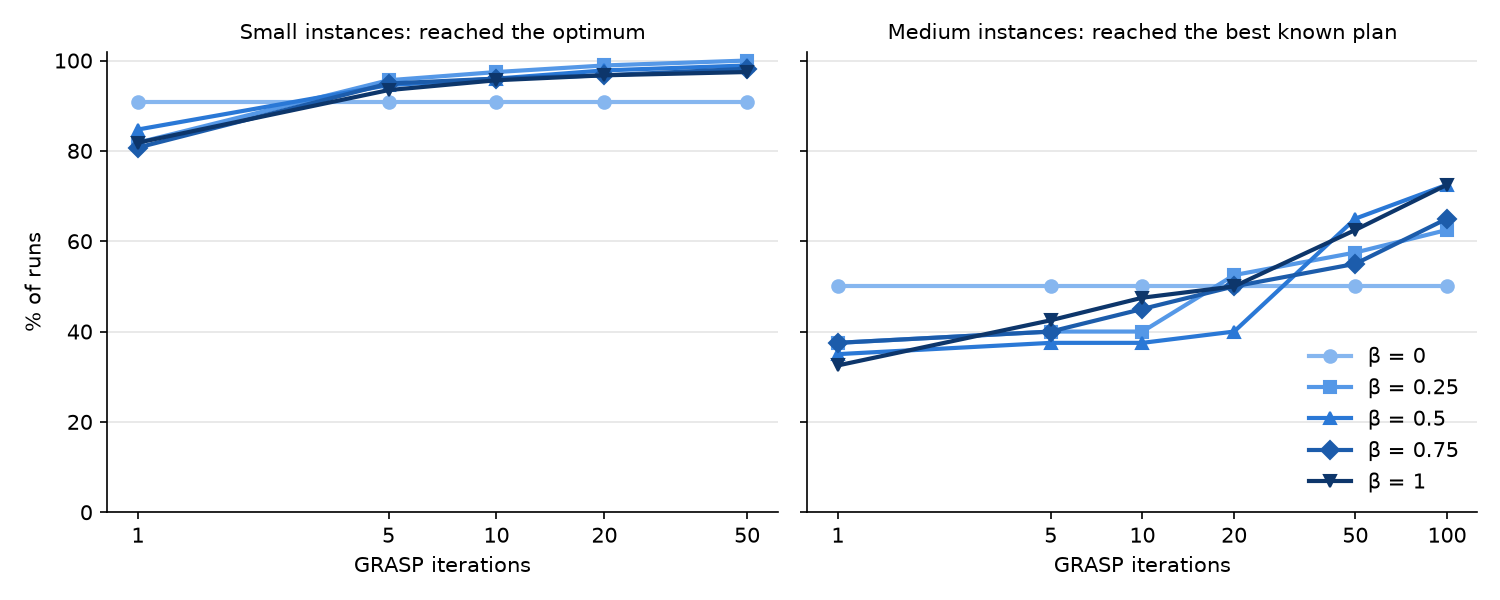
\includegraphics[width=\textwidth]{quality_vs_iterations.png}
  \caption{Share of runs that reach the optimum (small instances) or the best known plan
  (medium instances) after a given number of GRASP iterations, for each $\beta$.}
\end{figure}

Greedy construction ($\beta = 0$) is the best single iteration, but it builds the same plan every
time, so more iterations never help; on medium instances it is the only setting that loses on a
higher-priority goal ($f_3$, extra moves). Any $\beta > 0$ keeps improving with more iterations
and overtakes greedy after about 5 iterations (small) or 20--50 iterations (medium). No run with
$\beta > 0$ is worse than the best known plan on $f_1$--$f_3$; the remaining differences are in
coverage, on average 0.1\%. We use $\beta = 0.25$: it is the only value that reaches the optimum
in all small runs and has the smallest worst-case coverage gap on medium instances. $N = 100$
takes about 4~s on Edmonton, 7~s on Fez-Meknes case 1 and 13~s on case 2; on medium instances
quality is still rising at 100 iterations, so a larger $N$ or a time cap still pays off. The full
results (quality vs.\ time, runtimes) are reported in Section~6.

\paragraph{References.}
Feo, T.A., Resende, M.G.C. (1995). Greedy randomized adaptive search procedures.
\emph{Journal of Global Optimization} 6, 109--133.
Resende, M.G.C., Ribeiro, C.C. (2016). \emph{Optimization by GRASP}. Springer.

\end{document}
